\documentclass[12pt,a4paper]{article} 
\usepackage{tikz}
\usepackage{float}
\usepackage{graphicx}
\usepackage{multirow}
\usepackage{setspace} 
\usepackage{graphicx}
\usepackage{times}
\pagenumbering{roman}
\usepackage{geometry}

\geometry{verbose,tmargin=2cm,bmargin=2cm,lmargin=3cm,rmargin=2cm}
\usepackage{fancyhdr} 
%\linespread{1.05} 
\usepackage{tikz}
\usetikzlibrary{arrows}
\usetikzlibrary{shapes.geometric}

\tikzstyle{kres} = [rectangle, rounded corners, minimum width=1cm, minimum height=0.5cm,text centered, draw=black]
\tikzstyle{nad} = [trapezium, trapezium left angle=60, trapezium right angle=100, minimum width=1cm, minimum height=0.5cm, text centered, draw=black]
\tikzstyle{sim} = [trapezium, trapezium left angle=60, trapezium right angle=100, minimum width=1cm, minimum height=0.5cm, text centered, draw=black]
\tikzstyle{garis} = [thick,->,>=stealth]
\usetikzlibrary{shapes,arrows}

\begin{document} % Mulai Penulisan Laporan
\onehalfspacing
\begin{titlepage}

\title{\textbf{LAPORAN PRAKTIKUM ELEKTRONIKA DASAR
\\ OP-AMP INVERTING DAN NON-INVERTING}}  %Judul Laporan
%\title{\textbf{FOTOKATALISIS}}  %Judul Laporan
\author{\textbf {Dosen : Mada Sanjaya WS, Ph.D  }
\\ \textbf{Asisten Lab : Sri Rohmawati (1177030037)}
\\ \textbf{ }
\\ \textbf{Disusun Oleh :}
\\ \textbf{Muhamad Fahmi Adzkar} \textbf {(1187030024)}
\\ \textbf{Kelompok 3 :}
\\ \textbf{Hani Hikmawati} \textbf {(1187030014)}
\\ \textbf{Sri Rahayu} \textbf {(1187030036)}
\\ \textbf{Yuni Rahayu} \textbf {(1187030041)}}

\maketitle
\begin{center}
\vspace{1cm}

\includegraphics[width=4cm]{uin.png}
\vspace{1cm}

JURUSAN FISIKA\\
FAKULTAS SAINS DAN TEKNOLOGI\\
UIN SUNAN GUNUNG DJATI BANDUNG\\
2019\\
\end{center}
\end{titlepage}

\renewcommand\abstractname{Abstract} %Untuk Abstrak Bahasa Inggris
\begin{abstract} %Untuk Abstrak Bahasa Inggris
Experiments have been conducted on the Op-Amp Adder and Op-Amp Subtractor in the Advanced Physics Laboratory UIN Bandung with the aim of understanding the series of Adder and Subtractor, analyzing the working principle of the series of Adder and Subtractor, knowing the input and output waves in each circuit, and can calculate the output voltage in each circuit. From the result of the practicum, it was found that the output voltage 1 and the input 2 had a sense difference of 180 degrees in the waveform. The amount of output in the Op-Amp subtractor is a reduction of the input signal 1 and the input signal 2 and does not have a difference in taste so that the waveform is in tandem.

\textit{Keywords: Op-Amp, Adder, Subtractor}
\end{abstract}

\begin{abstract}
Telah dilakukan percobaan tentang Op-Amp Adder dan Op-Amp Subtractor di Laborstorium Advance Physics UIN bandung yang bertujuan untuk memahami rangkaian adder dan subtractor, menganalisa prinsip kerja rangkaian adder dan subtractor, mengetahui gelombang input dan output pada setiap rangkaian, dan menghitung tegangan output dari setiap rangkaian. Dari hasil praktikum, diperoleh bahwa besarnya tegangan output pada Op-Amp adder merupakan penjumlahan dari sinyal input 1 dan sinyal input 2 serta memiliki beda fasa sebesar 180 derajat pada bentuk gelombangnya. Besarnya tegangan output pada Op-Amp Subtractor merupakan pengurangan dari sinyal input 1 dan sinyal input 2 serta tidak memiliki beda fasa sehingga bentuk gelombangnya beriringan. 

\textit{Kata Kunci: Op-Amp, Adder, Subtractor }
\end{abstract}


\newpage
\section{PENDAHULUAN}
\paragraph{1.1 Latar Belakang}
\subparagraph{ }
	Penguat Operasional (Operasional Amplifier) atau yang biasa disebut Op-Amp merupakan suatu jenis penguat elektronika dengan hambatan (coupling) arus searah yang memiliki faktor penguatan sangat besar dengan dua masukan dan satu pengeluaran.
\subparagraph{ }
	Pada umumnya penguat operasional tersedia dalam bentuk sirkuit terpadu dan yang paling banyak digunakan adalah ranfkaian seri. Penguat opersional dalam rangkaian terpadu memiliki karakteristik yang mendekati karakteristik penguat operasional ideal tanpa perlu memperhatikan apa yang terdapat di dalamnya.
\subparagraph{ }
Penguat operasional adalah perangkat yang sangat efisien dan serba guna. Contoh penggunaan penguat operasional adalah untuk operasi matematika sederhana seperti penjumlahan dan pengurangan terhadap tegangan listrik hingga dikembangkan kepada penggunaan aplikatif seperti komparator dan osilator dengan distorsi rendah serta pengembangan alat komunikasi. Selain itu, aplikasi pemakaian op-amp juga meliputi bidang elektronika audio, pengatur tegangan DC, tapis aktif, penyearah presisi, pengubah analog digital dan pengubah digital ke analog, pengolah isyarat seperti cuplik tahan, penguat pengunci, kendali otomatik, computer analog, elektronika nuklir, dan lain-lain.

\paragraph{1.2 Tujuan}
\subparagraph{ }
Adapun tujuan dilakukannya praktikum ini yaitu:
\begin{enumerate}
\item Mampu memahami rangkaian adder dan subtractor.
\item Mampu menganalisa prinsip kerja rangkaian adder dan subtractor.
\item Mengetahui gelombang input dan output pada setiap rangkaian.
\item Dapat menghitung tegangan output dari setiap rangkaian.
\end{enumerate}


\newpage
\section{Landasan Teori}
\subsection{Dasar Teori}
\paragraph{ }
\textbf{1.Penguat operasional}
\subparagraph{ }
 Penguat operasional (bahasa Inggris: operational amplifier) atau yang biasa disebut op-amp merupakan suatu jenis penguat elektronika dengan sambatan (bahasa Inggris: coupling) arus searah yang memiliki bati (faktor penguatan atau dalam bahasa Inggris: gain) sangat besar dengan dua masukan dan satu keluaran.Penguat operasional pada umumnya tersedia dalam bentuk sirkuit terpadu dan yang paling banyak digunakan adalah seri 741.

Penguat operasional adalah perangkat yang sangat efisien dan serba guna.Contoh penggunaan penguat operasional adalah untuk operasi matematika sederhana seperti penjumlahan dan pengurangan terhadap tegangan listrik hingga dikembangkan kepada penggunaan aplikatif seperti komparator dan osilator dengan distorsi rendah.

Penguat operasional dalam bentuk rangkaian terpadu memiliki karakteristik yang mendekati karakteristik penguat operasional ideal tanpa perlu memperhatikan apa yang terdapat di dalamnya.Karakteristik penguat operasional ideal adalah:
\begin{enumerate}
\item Bati tegangan tidak terbatas.
\item Impedansi masukan tidak terbatas.
\item Impedansi keluaran nol.
\item Lebar pita tidak terbatas.
\item Tegangan offset nol (kondisi ketika masukan sebesar nol).
\end{enumerate}
	
\begin{flushright}
(Wikipedia.com)
\end{flushright}

\subparagraph{ }
\textbf{2.Komparator (pembanding)}
\subparagraph{ }
 Merupakan salah satu aplikasi yang memanfaatkan batas simpal terbuka (bahasa Inggris: open-loop gain) penguat operasional yang sangat besar.[5] Ada jenis penguat operasional khusus yang memang difungsikan semata-mata untuk penggunaan ini dan agak berbeda dari penguat operasional lainnya dan umum disebut juga dengan komparator (bahasa Inggris: comparator).

Komparator membandingkan dua tegangan listrik dan mengubah keluarannya untuk menunjukkan tegangan mana yang lebih tinggi.

$Vout = Vs+$   dimana   $V1>V2$   atau   $Vs-$   dimana   $V1<V2 $

\begin{flushright}
(Wikipedia.com) 
\end{flushright}

\paragraph{ }
\textbf{3.Penguat pembalik}
\subparagraph{ }
	Sebuah penguat pembalik menggunakan umpan balik negatif untuk membalik dan menguatkan sebuah tegangan.[12] Resistor Rf melewatkan sebagian sinyal keluaran kembali ke masukan.[12] Karena keluaran taksefase sebesar 180 derajat, maka nilai keluaran tersebut secara efektif mengurangi besar masukan.[12] Ini mengurangi bati keseluruhan dari penguat dan disebut dengan umpan balik negatif. Tanda negatif menunjukkan bahwa keluaran adalah pembalikan dari masukan.[12] Contohnya jika Rf adalah 10.000 ohm dan Rin adalah 1.000 ohm, maka nilai bati adalah -10.000 ohm / 1.000 ohm,, yaitu -10.
	
\begin{flushright}
(Wikipedia.com) 
\end{flushright}
	
\subparagraph{ }
\textbf{4.Penguat non-pembalik}
\subparagraph{ }
	Dengan demikian, penguat non-pembalik memiliki bati minimum bernilai 1. Karena tegangan sinyal masukan terhubung langsung dengan masukan pada penguat operasional maka impedansi masukan bernilai tak hingga.
	
\begin{flushright}
(Wikipedia.com) 
\end{flushright}

\paragraph{ }
\textbf{Pengertian Op-Amp (Operational Amplifier)}
\subparagraph{ }
	Pengertian Op-Amp (Operational Amplifier) – Operational Amplifier atau lebih dikenal dengan istilah Op-Amp adalah salah satu dari bentuk IC Linear yang berfungsi sebagai Penguat Sinyal listrik. Sebuah Op-Amp terdiri dari beberapa Transistor, Dioda, Resistor dan Kapasitor yang terinterkoneksi dan terintegrasi sehingga memungkinkannya untuk menghasilkan Gain (penguatan) yang tinggi pada rentang frekuensi yang luas. Dalam bahasa Indonesia, Op-Amp atau Operational Amplifier sering disebut juga dengan Penguat Operasional.


 
Op-Amp umumnya dikemas dalam bentuk IC, sebuah IC Op-Amp dapat terdiri dari hanya 1 (satu) rangkaian Op-Amp atau bisa juga terdiri dari beberapa rangkaian Op-Amp. Jumlah rangkaian Op-Amp dalam satu kemasan IC dapat dibedakan menjadi Single Op-Amp, dual Op-Amp dan Quad Op-Amp. Ada juga IC yang didalamnya terdapat rangkaian Op-Amp disamping rangkaian utama lainnya.

Sebuah rangkaian Op-Amp memiliki dua input (masukan) yaitu satu Input Inverting dan satu Input Non-inverting serta memiliki satu Output (keluaran). Sebuah Op-Amp juga memiliki dua koneksi catu daya yaitu satu untuk catu daya positif dan satu lagi untuk catu daya negatif. Bentuk Simbol Op-Amp adalah Segitiga dengan garis-garis Input, Output dan Catu dayanya seperti pada gambar dibawah ini. Salah satu tipe IC Op-Amp yang populer adalah IC741.

\begin{flushright}
(https://teknikelektronika.com) 
\end{flushright}

\paragraph{ }
\textbf{Karakteristik Op-Amp (Operational Amplifier)}
\subparagraph{ }
Karakteristik Faktor Penguat atau Gain pada Op-Amp pada umumnya ditentukan oleh Resistor Eksternal yang terhubung diantara Output dan Input pembalik (Inverting Input). Konfigurasi dengan umpan balik negatif (Negative Feedback) ini biasanya disebut dengan Closed-Loop configuration atau Konfigurasi Lingkar Tertutup. Umpan balik negatif ini akan menyebabkan penguatan atau gain menjadi berkurang dan menghasilkan penguatan yang dapat diukur serta dapat dikendalikan. Tujuan pengurangan Gain dari Op-Amp ini adalah untuk menghindari terjadinya Noise yang berlebihan dan juga untuk menghindari respon yang tidak diinginkan. Sedangkan pada Konfigurasi Lingkar Terbuka atau Open-Loop Configuration, besar penguatannya adalah tak terhingga $(tak terhingga)$ sehingga besarnya tegangan output hampir atau mendekati tegangan Vcc.

Secara umum, Operational Amplifier (Op-Amp) yang ideal memiliki karakteristik sebagai berikut :
\begin{enumerate}
\item Penguatan Tegangan Open-loop atau $Av = (tak terhingga)$
\item Tegangan Offset Keluaran (Output Offset Voltage) $atau Voo = 0 (nol)$
\item Impedansi Masukan (Input Impedance) atau $Zin=(tak terhingga)$
\item Impedansi Output (Output Impedance ) $atau Zout = 0 (nol)$
\item Lebar Pita (Bandwidth) atau $BW =(tak terhingga)$
\item Karakteristik tidak berubah dengan suhu
\end{enumerate}

Pada dasarnya, kondisi Op-Amp ideal hanya merupakan teoritis dan hampir tidak mungkin dicapai dalam kondisi praktis. Namun produsen perangkat Op-Amp selalu berusaha untuk memproduksi Op-Amp yang mendekati kondisi idealnya ini. Oleh karena itu, sebuah Op-Amp yang baik adalah Op-Amp yang memiliki karakteristik yang hampir mendekati kondisi Op-Amp Ideal.


 


\begin{flushright}
(https://Wikipedia.com) 
\end{flushright}

\paragraph{ }
\textbf{Komparator Op-amp}
\subparagraph{ }
	Komparator Op-amp membandingkan satu level tegangan analog dengan level tegangan analog lainnya, beberapa tegangan Referensi Preset, Vref dan menghasilkan sinyal output berdasarkan perbandingan tegangan. Komparator tegangan Op-amp membandingkan besaran dua input tegangan dan menentukan yang mana yang terbesar dari keduanya. Penguat Operasional Standar dicirikan oleh Gain Loop Terbuka AO dan bahwa tegangan outputnya.
	
	\begin{center}
	$ Vout = AO (V+ - V-)$
	\end{center}
	Dimana: V+ dan V- tegangan pada terminal - membalikkan dan membalik.

Pembanding tegangan, baik menggunakan umpan balik positif atau tidak ada umpan balik sama sekali (Mode Loop Terbuka) untuk mengalihkan outputnya di antara dua kondisi jenuh, karena dalam mode loop terbuka penguat gain tegangan pada dasarnya sama dengan AVO. Karena Gain Loop Terbuka yang tinggi, output dari komparator mengayun sepenuhnya ke rel pasokan positifnya, +Vcc atau sepenuhnya ke rel pasokan negatifnya, -Vcc pada aplikasi berbagai sinyal input yang melewati beberapa nilai ambang yang telah ditetapkan. Pembanding op-amp dasar menghasilkan output tegangan positif atau negatif dengan membandingkan tegangan inputnya terhadap beberapa tegangan referensi DC yang telah ditetapkan. Pembagi tegangan resistif digunakan untuk mengatur tegangan referensi input dari komparator, tetapi sumber baterai, dioda zener atau potensiometer untuk tegangan referensi variabel. Secara teori tegangan referensi pembanding diatur untuk berada di mana saja antara 0V dan tegangan suplai tetapi ada batasan pada rentang tegangan yang sebenarnya tergantung pada komparator op-amp yang digunakan.
	
\begin{flushright}
(http://myelectronicnote.blogspot.com) 
\end{flushright}


\newpage
\section{METODE PRAKTIKUM}
\subsection{Waktu dan Tempat}
\paragraph{ }
Praktikum ini dilaksanakan pada:
\\ 		Tanggal : jum'at, 29 November 2019
\\ 		Waktu : 07.00 WIB - Selesai
\\ 		Tempat : Advance Physics 


\subsection{Alat dan Bahan}
Alat dan bahan yang digunakan dalam praktikum ini diantaranya adalah : 
\subparagraph*{ }
\begin{tabular}{|l|l|l|}  \hline
No & Alat dan Bahan  & Jumlah  \\ \hline
1  & Projek board & 1 Buah \\ \hline
2  & IC LM741 & satu set \\ \hline
3  & Baterai 9 volt & Secukupnya \\ \hline
4  & Kancing Baterai 3 Pin & 1 Buah \\ \hline
5  & Kabel Tunggal  & Secukupnya \\ \hline
6  & Resistor  & 2 Buah \\ \hline
7  & Multimeter & Satu set \\ \hline
8  & Osiloskop & Satu set \\ \hline
\end{tabular}

  
    
\subsection{Prosedur Percobaan}
\subparagraph{3.3.1 Percobaan Rangkaian Inverting }
\subparagraph{ }
\textbf{Rangkaian Inverting} Rangkaian disusun sesuai dengan gambar di lampiran dan project board. Kemudian siapkan alat dan bahan yang digunakan. Kemudian Susun rangkaian sesuai dengan gambar simulasi di papan tulis. kemudian ukur besar resistansi pada resistor. Dilanjut dengan diukurnya besar tegangan pada rangkaian inverting dan ketika diberikan tegangan sebesar 9 V arus DC, diukur  V pada rangkaian inverting ketika kondisi stabil di osiloskop. kemudian data ditulis pada tabel.
	
\subparagraph{3.3.2 Percobaan Rangkaian Non-Inverting }
\subparagraph{ }
	\textbf{Rangkaian Non-Inverting} Rangkaian disusun sesuai dengan gambar di lampiran dan project board. Kemudian siapkan alat dan bahan yang digunakan. Kemudian Susun rangkaian sesuai dengan gambar simulasi di papan tulis. kemudian ukur besar resistansi pada resistor. Dilanjut dengan diukurnya besar tegangan pada rangkaian inverting dan ketika diberikan tegangan sebesar 9 V arus DC, diukur  V pada rangkaian inverting ketika kondisi stabil di osiloskop. kemudian data ditulis pada tabel.

\subsection{Diagram Alir}
\subsubsection{Percobaan Rangkaian Inverting }
\tikzstyle{line} = [draw, -latex']
\tikzstyle{cloud} = [draw, rectangle,fill=blue!20, node distance=3cm,
    minimum height=0.7cm]
\tikzstyle{kres} = [draw, rectangle, rounded corners,fill=blue!20, node distance=3cm,
    minimum height=0.7cm]
\begin{tikzpicture}[node distance = 1.3cm, auto]
    % Place nodes
       \node [kres] (a) {Siapkan alat dan bahan yang digunakan};
       \node [cloud, below of = a , node distance = 1.5cm] (b) {Susun rangkaian sesuai dengan gambar};         
       \node [cloud, below of = b , node distance = 1.5cm] (c) {Mengukur nilai resistansi pada resistor};
       \node [cloud, below of = c , node distance = 1.5cm] (d) {Masukan tegangan Baterai 9 Volt DC};
       \node [cloud, below of = d , node distance = 1.5cm] (e) {Mengukur V output dengan osiloskop ketika kondisi gelombang stabil};        
       \node [cloud, below of = e , node distance = 1.5cm] (f) {Hasil data ditulis pada tabel};
        
        
     % Draw edges
    \path [line] (a) -- (b);
    \path [line] (b) -- (c);
    \path [line] (c) -- (d);
    \path [line] (d) -- (e);
    \path [line] (e) -- (f);
    \end{tikzpicture}   

	\subsubsection{Percobaan Rangkaian Non-Inverting }
\tikzstyle{line} = [draw, -latex']
\tikzstyle{cloud} = [draw, rectangle,fill=blue!20, node distance=3cm,
    minimum height=0.7cm]
\tikzstyle{kres} = [draw, rectangle, rounded corners,fill=blue!20, node distance=3cm,
    minimum height=0.7cm]
\begin{tikzpicture}[node distance = 1.3cm, auto]
    % Place nodes
       \node [kres] (a) {Siapkan alat dan bahan yang digunakan};
       \node [cloud, below of = a , node distance = 1.5cm] (b) {Susun rangkaian sesuai dengan gambar};         
       \node [cloud, below of = b , node distance = 1.5cm] (c) {Mengukur nilai resistansi pada resistor};
       \node [cloud, below of = c , node distance = 1.5cm] (d) {Masukan tegangan Baterai 9 Volt DC};
       \node [cloud, below of = d , node distance = 1.5cm] (e) {Mengukur V output dengan osiloskop ketika kondisi gelombang stabil};        
       \node [cloud, below of = e , node distance = 1.5cm] (f) {Hasil data ditulis pada tabel};
        
     % Draw edges
    \path [line] (a) -- (b);
    \path [line] (b) -- (c);
    \path [line] (c) -- (d);
    \path [line] (d) -- (e);
    \path [line] (e) -- (f);
    \end{tikzpicture}   

\newpage

\section{Data dan Pembahasan}

\subsection{Data Hasil Pengamatan}
\paragraph{ } Setelah melakukan eksperimen, maka didapatkan hasil percobaan sebagai berikut.

\subparagraph*{$\bullet$ Rangkaian Percobaan Inverting }
\subparagraph*{ }
\begin{tabular}{|c|c|c|c|c|c|c|c|c|c|c|}        \hline
No & Ri       & Rf       & Gain      & Vin       &Vout            \\ \hline 
1. & 5,6 Kohm & 9,8 Kohm & 1,75 Kohm & 0,4 Volt  & 0,2 Volt       \\ \hline
 \end{tabular}
 
\subparagraph*{$\bullet$ Rangkaian Percobaan Non-Inverting }
\subparagraph*{ }
\begin{tabular}{|c|c|c|c|c|c|c|c|c|c|c|}        \hline
No & Ri       & Rf       & Gain      & Vin       & Vout            \\ \hline 
1. & 1,1 Kohm & 5,6 Kohm & 6,09 Kohm & 0,6 Volt  & 8 Volt \\ \hline
 \end{tabular}




\newpage
\subsection{Pembahasan}
\subparagraph{ }
	Berdasarkan praktikum yang telah dilakukan, maka dapat diketahui bahwa prinsip kerja IC LM741 pada rangkaian Injverting memiliki dua karakteristik. yaitu jika arus yang masuk melalui Va (negatif) maka akan menjadi penguat pembalik dan pada osiloskop akan memberikan sinyal sinusoidal negatif. Sedangkan sebaliknya, jika arus yang masuk melalui Vb (positif) maka akan menjadi penguat dan pada osiloskop akan memberikan sinyal sinusoidal positif.
	Berdasarkan hasil yang telah dilakukan dengan Hardware. Pada rangkaian percobaan Inverting, didapatkan bahwa Tegangan masuk (Vin) bernilai 0,4 Volt (ketika mengamati tegangan di Osiloskop) dan Tegangan keluar (Vout) bernilai 0,2 Volt (ketika mengamati tegangan di Osiloskop). Menurut hipotesa praktikan hal tersebut dapat terjadi karena perbedaan resistansi yang cukup jauh karena Ri bernilai 5,6 Kohm sedangkan Rf bernilai 9,8 Kohm. Namun perbedaan nilai arus-arus tersebut tidak terlalu besar yaitu hanya sedikit.Dan nilai Gain yang di dapat adalah 1,75 Kohm. Maka dari itu hasil dari praktikum ini hampir sesuai dengan teori hukum penguat inverting.
\subparagraph{ }
	Berdasarkan hasil yang telah dilakukan dengan Hardware. Pada rangkaian percobaan Inverting, didapatkan bahwa Tegangan masuk (Vin) bernilai 0,6 Volt (ketika mengamati tegangan di Osiloskop) dan Tegangan keluar (Vout) bernilai 8 Volt (ketika mengamati tegangan di Osiloskop). Menurut hipotesa praktikan hal tersebut dapat terjadi karena perbedaan resistansi yang cukup jauh karena Ri bernilai 1,1 Kohm sedangkan Rf bernilai 5,6 Kohm. Namun perbedaan nilai arus-arus tersebut tidak terlalu besar yaitu hanya sedikit.Dan nilai Gain yang di dapat adalah 6,09 Kohm. Maka dari itu hasil dari praktikum ini hampir sesuai dengan teori hukum penguat inverting.
\newpage
 
\subsection{Analisis Data}
\subparagraph{}
	Hasil praktikum ini bisa dinyatakan berhasil tidaknya dapat dilihat dari hasil data, jika besar tegangan (vin) yang dihasilkan tidak beda jauh dan bernilai sama dengan hasil perhitungan teori dan jika besar tegangan (vout) yang dihasilkan tidak beda jauh dan bernilai sama dengan hasil perhitungan teori maka itu dapat dikatakan berhasil. adapun faktor yang mempengaruhi hasil kesalahan-kesalahan pada saat praktikum yaitu pada saat pengolahan data dan juga pada saat pengambilan data pada saat menggunakan alat.
 

\newpage
\section{Kesimpulan}
\subparagraph{ }
Dari praktikum ini dapat disimpulkan bahwa :
\begin{enumerate}

\item Operational Amplifier atau lebih dikenal dengan istilah Op-Amp adalah salah satu dari bentuk IC Linear yang berfungsi sebagai Penguat Sinyal listrik. Sebuah Op-Amp terdiri dari beberapa Transistor, Dioda, Resistor dan Kapasitor yang terinterkoneksi dan terintegrasi sehingga memungkinkannya untuk menghasilkan Gain (penguatan) yang tinggi pada rentang frekuensi yang luas. Dalam bahasa Indonesia, Op-Amp atau Operational Amplifier sering disebut juga dengan Penguat Operasional.

\item Penguat operasional (bahasa Inggris: operational amplifier) atau yang biasa disebut op-amp merupakan suatu jenis penguat elektronika dengan sambatan (bahasa Inggris: coupling) arus searah yang memiliki bati (faktor penguatan atau dalam bahasa Inggris: gain) sangat besar dengan dua masukan dan satu keluaran. Penguat operasional pada umumnya tersedia dalam bentuk sirkuit terpadu dan yang paling banyak digunakan adalah seri 741.
Penguat operasional adalah perangkat yang sangat efisien dan serba guna. Contoh penggunaan penguat operasional adalah untuk operasi matematika sederhana seperti penjumlahan dan pengurangan terhadap tegangan listrik hingga dikembangkan kepada penggunaan aplikatif seperti komparator dan osilator dengan distorsi rendah.

\item Op-Amp umumnya dikemas dalam bentuk IC, sebuah IC Op-Amp dapat terdiri dari hanya 1 (satu) rangkaian Op-Amp atau bisa juga terdiri dari beberapa rangkaian Op-Amp. Jumlah rangkaian Op-Amp dalam satu kemasan IC dapat dibedakan menjadi Single Op-Amp, dual Op-Amp dan Quad Op-Amp. Ada juga IC yang didalamnya terdapat rangkaian Op-Amp disamping rangkaian utama lainnya.

\item Karakteristik Faktor Penguat atau Gain pada Op-Amp pada umumnya ditentukan oleh Resistor Eksternal yang terhubung diantara Output dan Input pembalik (Inverting Input). Konfigurasi dengan umpan balik negatif (Negative Feedback) ini biasanya disebut dengan Closed-Loop configuration atau Konfigurasi Lingkar Tertutup. Umpan balik negatif ini akan menyebabkan penguatan atau gain menjadi berkurang dan menghasilkan penguatan yang dapat diukur serta dapat dikendalikan. Tujuan pengurangan Gain dari Op-Amp ini adalah untuk menghindari terjadinya Noise yang berlebihan dan juga untuk menghindari respon yang tidak diinginkan. Sedangkan pada Konfigurasi Lingkar Terbuka atau Open-Loop Configuration, besar penguatannya adalah tak terhingga $(tak terhingga)$ sehingga besarnya tegangan output hampir atau mendekati tegangan Vcc.

\end{enumerate}

\newpage
\begin{thebibliography}{99} % Daftar Pustaka
\bibitem{1} {Nave, Carl Rod (2006). "HyperPhysics - Operational Amplifier" (dalam bahasa Inggris). Department of Physics and Astronomy, Georgia State University. Diakses tanggal 2010-05-08. }

\bibitem{2} {Terjemahan istilah berdasarkan: "Glosarium". Pusat Bahasa Departemen Pendidikan Nasional. Diakses tanggal 2010-05-08.}

\bibitem{3} {Carter, Bruce; Brown, Thomas. "Handbook of Operational Amplifier Applications" (PDF). Texas Instruments. Diakses tanggal 2010-05-15}

\bibitem{4} {Tipler, Paul A., 1998 ”‘Fisika untuk Sains dan Teknik” .Jakarta : Erlangga }

\end{thebibliography}

\newpage
\begin{center}
\large{\textbf{LAMPIRAN}}
\end{center}

\newpage
\begin{figure}
\paragraph{Gambar percobaan}
\paragraph{ }
\begin{center}

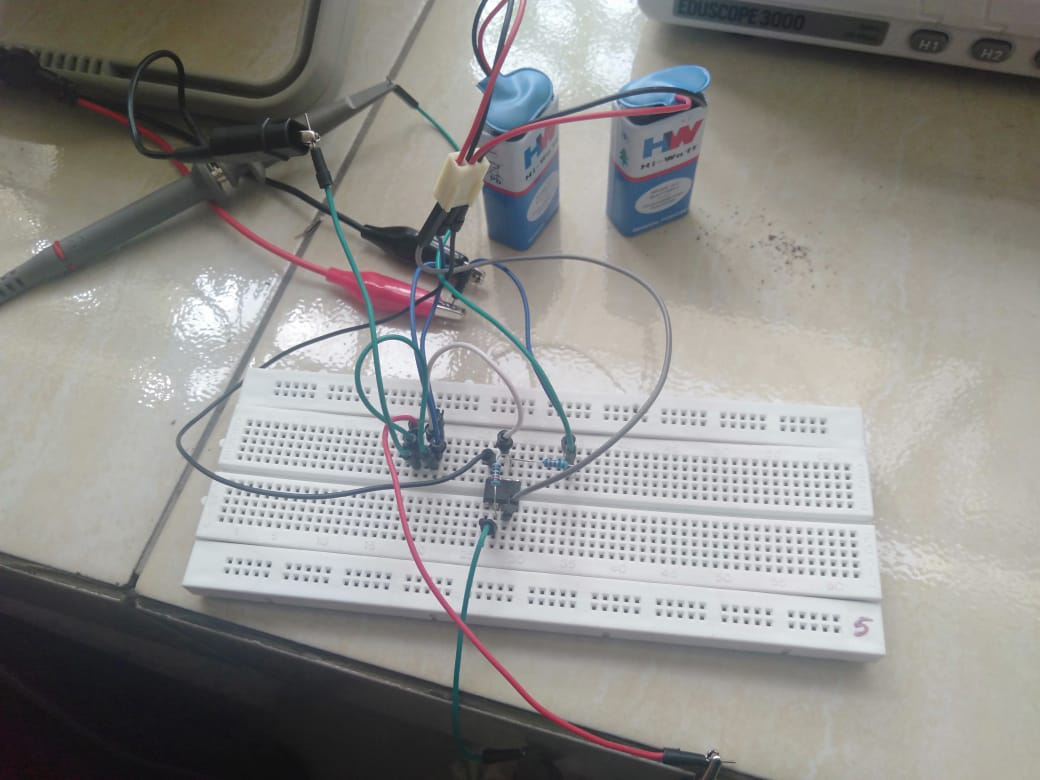
\includegraphics[width=12cm, height=5cm]{inverting1.png}

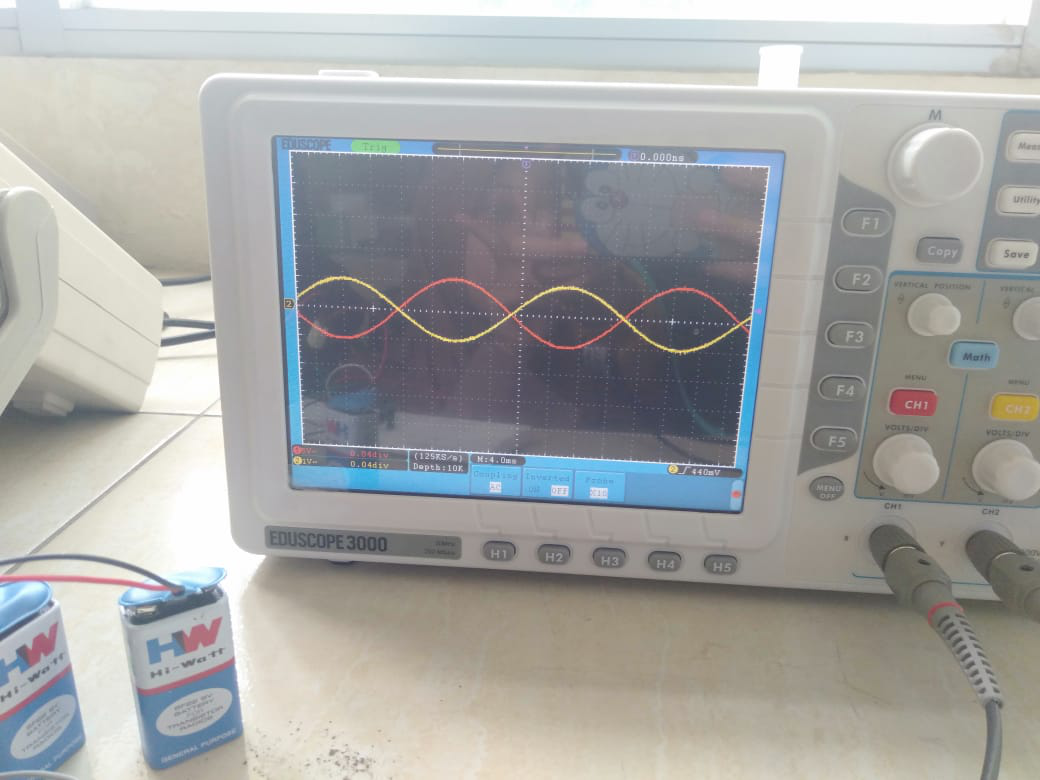
\includegraphics[width=12cm, height=6cm]{inverting2.png}

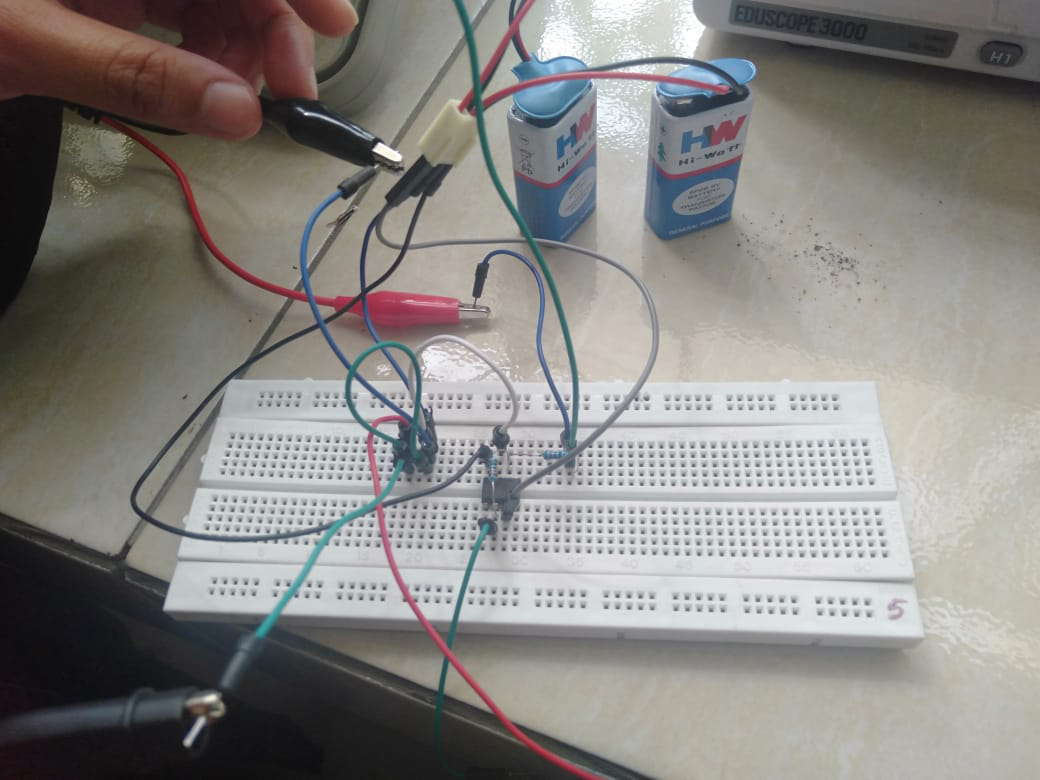
\includegraphics[width=12cm, height=6cm]{inverting3.png}
\end{center}
\end{figure}
\vspace{2cm}

\newpage
\begin{figure}
\paragraph{Gambar percobaan inverting dan non-inverting}
\paragraph{ }
\begin{center}

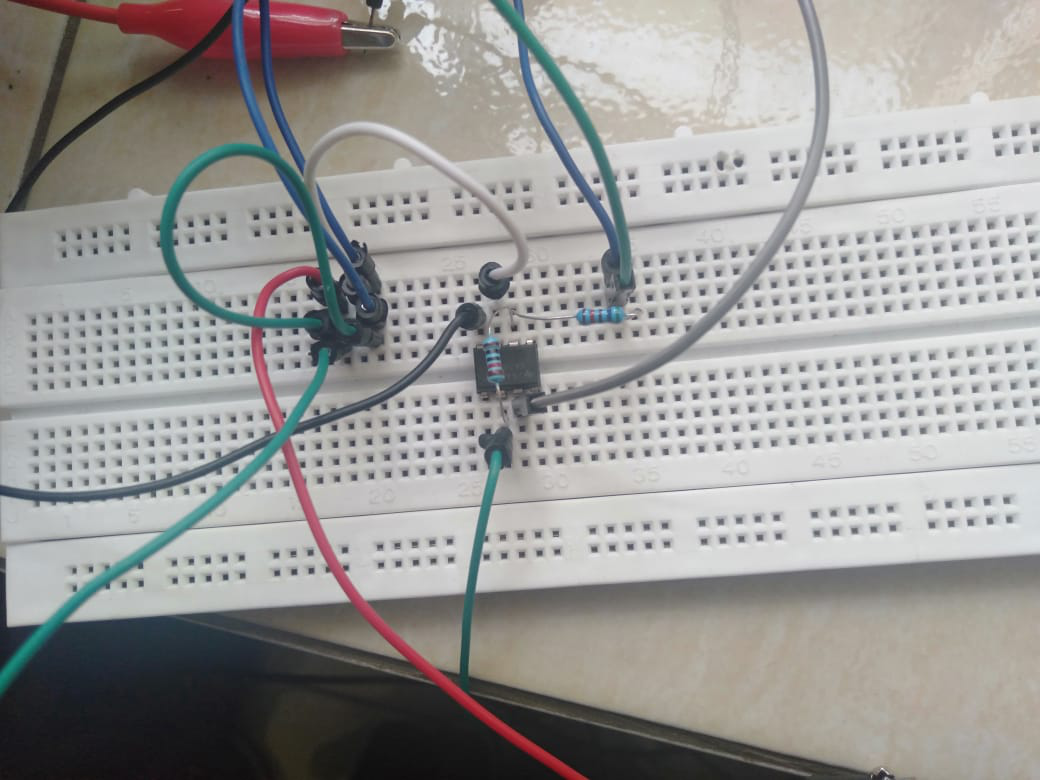
\includegraphics[width=12cm, height=5cm]{inverting4.png}

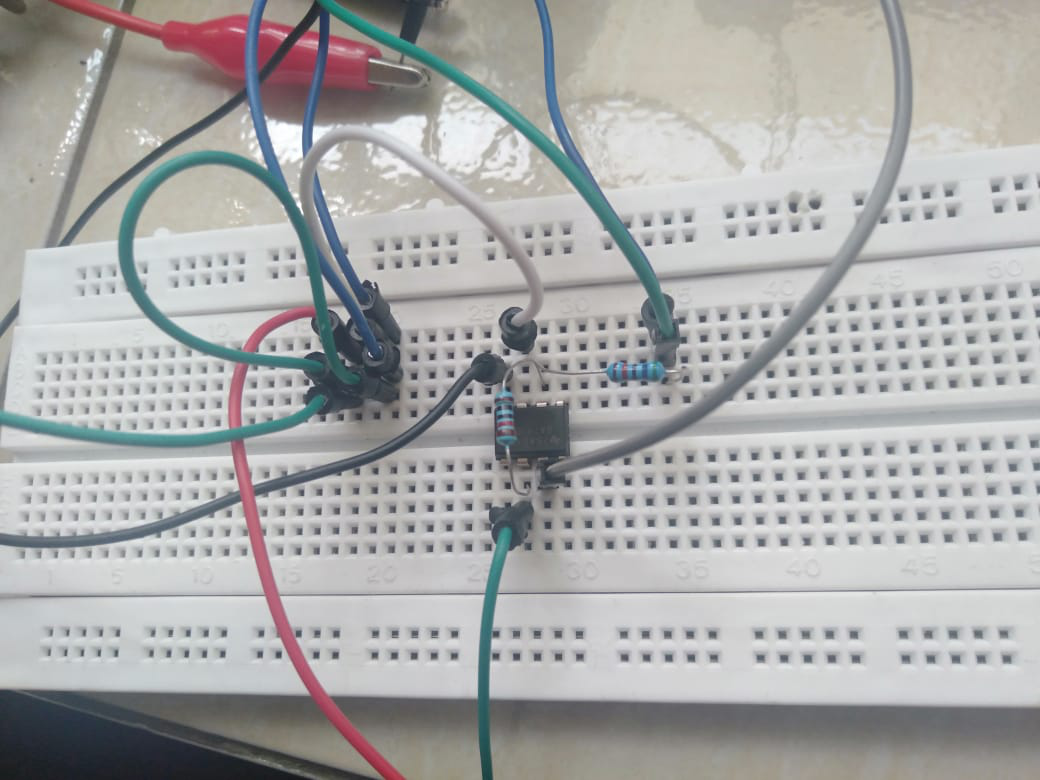
\includegraphics[width=12cm, height=6cm]{inverting5.png}

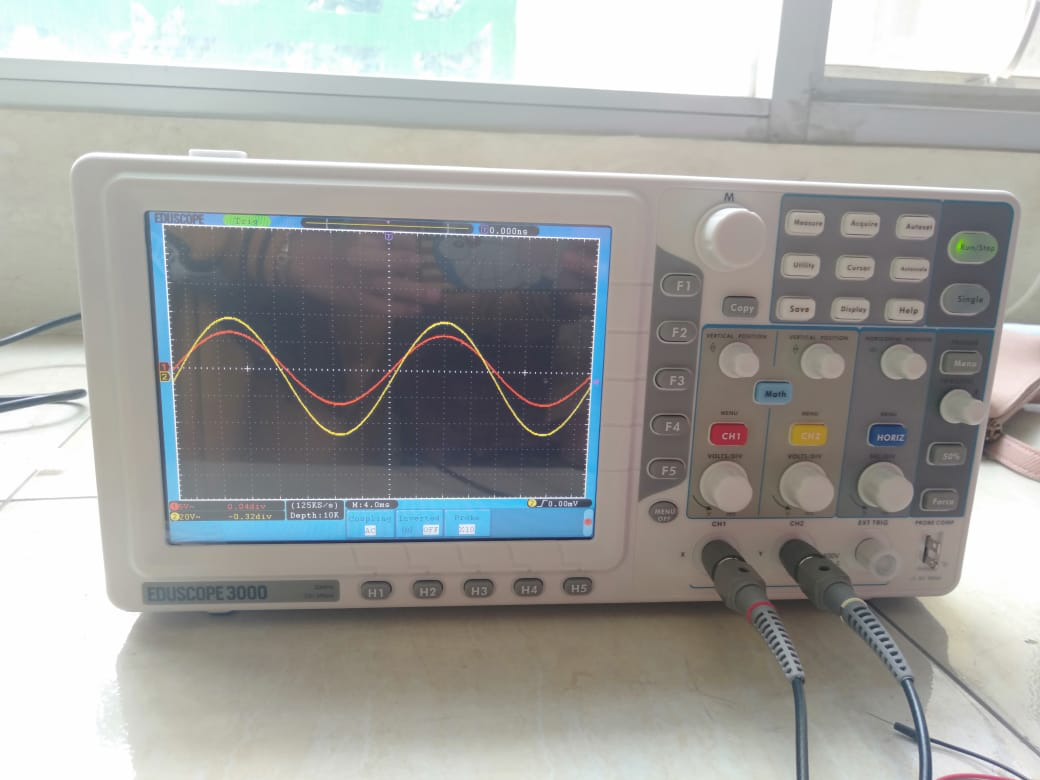
\includegraphics[width=12cm, height=6cm]{noninverting3.png}

\end{center}
\end{figure}
\vspace{2cm}

\newpage
\begin{figure}
\paragraph{Gambar percobaan non-inverting}
\paragraph{ }
\begin{center}

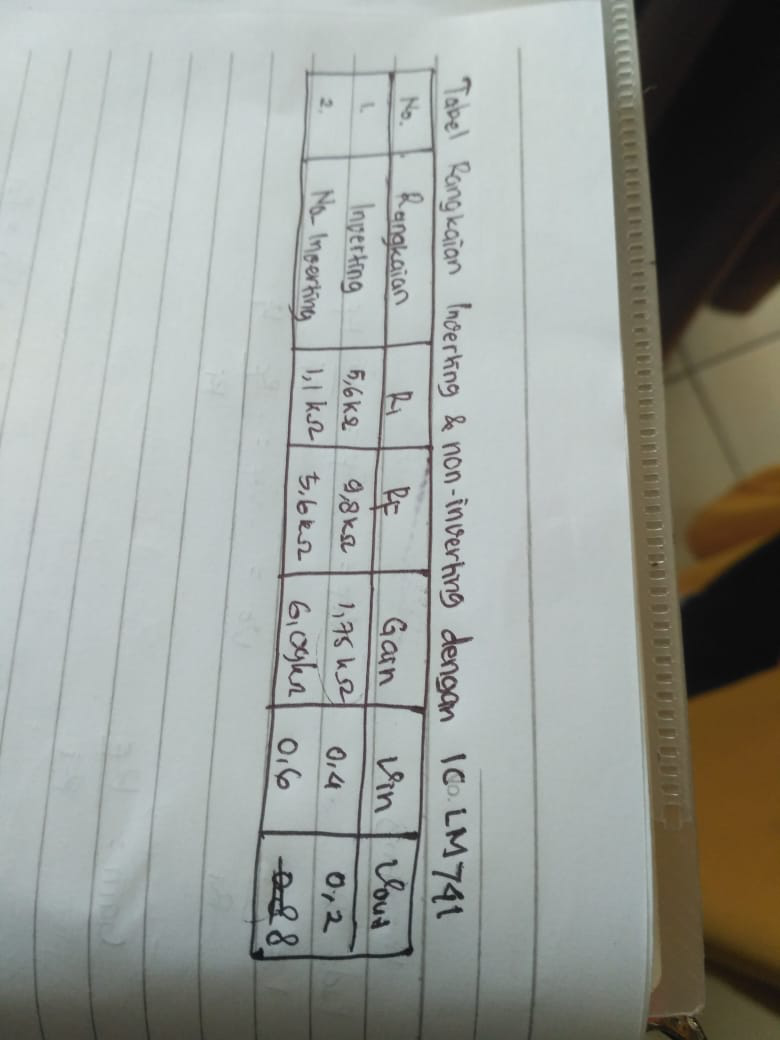
\includegraphics[width=6cm, height=12cm]{noninverting1.png}

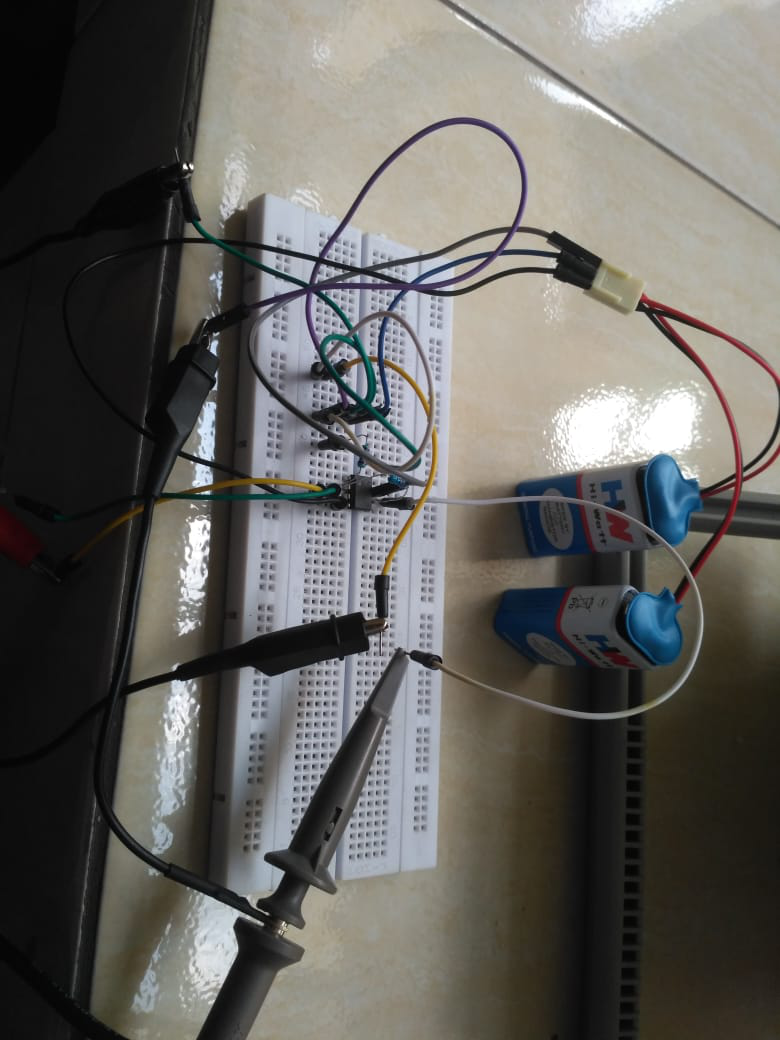
\includegraphics[width=6cm, height=12cm]{noninverting2.png}

\end{center}
\end{figure}
\vspace{2cm}

\end{document} %Penulisan Laporan Berakhir
